% http://www.ctan.org/tex-archive/macros/latex/contrib/beamer/examples
% http://latex.artikel-namsu.de/english/beamer-examples.html

\documentclass{beamer}
\usepackage{amsmath}
\usepackage{amssymb}
\usepackage{bm}
\usepackage{fancybox, graphicx}
\usepackage{listings}


\lstdefinestyle{customc}{
  belowcaptionskip=1\baselineskip,
  breaklines=true,
  %frame=L,
  xleftmargin=\parindent,
  language=bash,
  showstringspaces=false,
  basicstyle=\footnotesize\ttfamily,
  keywordstyle=\bfseries\color{green!40!black},
  commentstyle=\itshape\color{purple!40!black},
  identifierstyle=\color{blue},
  stringstyle=\color{orange},
}

\lstset{style=customc}

\usetheme{Warsaw}


\title[HPC Workshop] % (optional, use only with long paper titles)
{HPC Workshop}

\author[Balan,Whiteway] % (optional, use only with lots of authors)
{S.~T.~Balan,L.~Whiteway}

\institute[UCL]
{
  Department of Physics and Astronomy\\
  University College London
}
\date[HPC 2015]
{October 2014}

\subject{ HPC}

\begin{document}

\frame{\titlepage}

\section{Basics}

\begin{frame}{How to access training materials?}
  \begin{block}{url}
    \url{https://github.com/Astrophysics-UCL/HPCInfo/tree/master/training/linux_hpc_workshop_oct_2014}
  \end{block}
\end{frame}


\begin{frame}{What will you learn?}
  \begin{itemize}
    \item Accessing Astrophysics group machines
    \item Using linux console for your research
    \item Running your programs in HPC machines
  \end{itemize}
\end{frame}

\begin{frame}[fragile]{Accessing machines from outside}
  \alert{You will need a \emph{username} and \emph{password}}
  \begin{block}{steps}
    \lstinputlisting{commands/login.sh}
  \end{block}
\end{frame}

\begin{frame}[fragile]{command structure}
  \begin{block}{structure}
    \lstinputlisting{commands/command.sh}
  \end{block}
  \begin{example}
    \lstinputlisting{commands/command_example.sh}
  \end{example}
\end{frame}



\begin{frame}{HPC Facilities}
  \begin{table}
    \begin{tabular}{|c|c|c|c|}
      \hline
      machine & type & cores & memory  \\
      \hline
      \textsc{splinter}-1 & distributed & 96 & 48GB  \\
      \textsc{splinter}-2 & shared & 40 & 1TB \\
      \textsc{phalanx} & shared & 32 & 512GB \\
      \hline
    \end{tabular}
  \end{table}
\end{frame}

\begin{frame}{\textsc{splinter} distributed}
  \begin{figure}
    \begin{center}
      \shadowbox{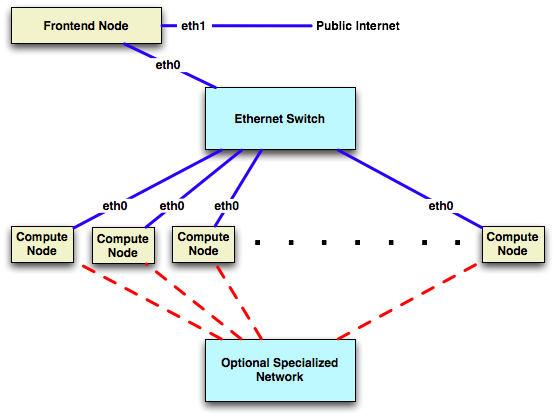
\includegraphics[scale=0.4]{img/cluster.png}}
      \footnote{\url{http://www.rocksclusters.org/}}
    \end{center}
  \end{figure}
\end{frame}

\begin{frame}{\textsc{splinter} shared}
  \begin{figure}
    \begin{center}
      \shadowbox{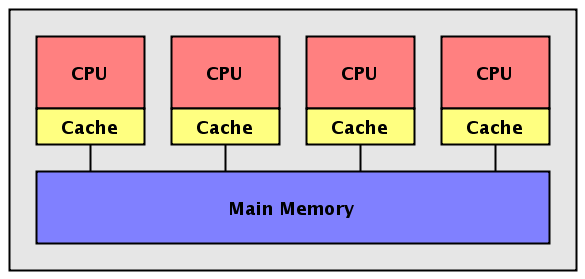
\includegraphics[scale=0.4]{img/fig03.png}}
      \footnote{\url{http://www.cs.rit.edu/}}
    \end{center}
  \end{figure}
\end{frame}

\begin{frame}{Best practices I}
  \begin{itemize}
    \item Choose the machines that are suited for your problem
    \item Read the User Guide
    \item Do not run your programs in the login node
    \item Do not install common software locally
    \item Request optimum resouces
    \item Minimise data transfer between nodes,
    \item \alert{Backup! Backup! Backup!}
  \end{itemize}
\end{frame}

\begin{frame}[fragile]{Submitting jobs}
  \fontsize{9pt}{9}\selectfont
  \begin{columns}
    \column{.3\textwidth}
    \begin{block}{commands}
      \lstinputlisting{commands/job_submission.sh}
    \end{block}

    \column{0.7\textwidth}
    \begin{example}
      \lstinputlisting{commands/sample_job_script.sh}
    \end{example}
  \end{columns}
\end{frame}

\begin{frame}{Exercises III}
  \fontsize{10pt}{8}\selectfont
  \begin{enumerate}
    \item Login to your HCP machine and find the path to your \texttt{HOME}
    directory and your quota
    \item Find the processor type and the version of your operating system
    \item Request an interative \texttt{queue} and run the \texttt{hello\_world.exe}
    \item Sumbit \texttt{hello\_world.exe} using a job script, find its \texttt{jobid}, check the output log.
    \item Compile \texttt{big\_mem\_example}, submit it using a \texttt{job-script} and see how much menory it uses
    \item Compile \texttt{time\_pause\_example}, submit it using a \texttt{job-script} and kill this job using its \texttt{jobid}.
    \item In the previous example see what happens when you play with the time requested.
  \end{enumerate}
\end{frame}


\begin{frame}{More information}
  \begin{block}{ap-wiki}
    \url{http://www.ucl.ac.uk/star/GroupAWiki}
  \end{block}

  \begin{block}{UCL Research Computing Platforms}
    \url{https://wiki.rc.ucl.ac.uk/wiki/Main_Page}
  \end{block}

  \begin{block}{DiRAC}
    \url{http://www.dirac.ac.uk/}
  \end{block}
\end{frame}


\end{document}
